\documentclass[11pt]{article}

\usepackage[utf8]{inputenc}
\usepackage[spanish]{babel}
\usepackage{enumerate}
\usepackage{float}
\usepackage[hidelinks]{hyperref}
\usepackage{graphicx}
\usepackage{minted}
\usepackage[vmargin=2.3cm,hmargin=2.3cm]{geometry}
\newcommand{\horrule}[1]{\rule{\linewidth}{#1}}
\usepackage{graphicx}


%----------------------------------------------------------------------------------------
%	Portada
%----------------------------------------------------------------------------------------
\title{	
	\normalfont \normalsize 
	\textsc{\textbf{Estructura de datos (2016-2017)} \\ Grado en Ingeniería Informática \\ Universidad de Granada} \\ [25pt] 
	\horrule{0.5pt} \\[0.4cm]
	\huge Práctica I: Eficiencia de los algoritmos \\ 
	\horrule{2pt} \\[0.5cm] 
}

\author{Elena María Gómez Ríos} 
%----------------------------------------------------------------------------------------


\begin{document}
\maketitle
\thispagestyle{empty}

\newpage
\tableofcontents
\thispagestyle{empty}
\newpage


\section{Realizar el análisis de eficiencia cuando consideramos el código en ocurrencias.cpp.}

Vamos a obtener la eficiencia teórica del código de \texttt{ocurrencias.cpp}. Como se puede observar la mayor parte del tiempo de ejecución se emplea en el método \texttt{contar\_hasta}, el cual es de orden $0(n)$.
\begin{minted}{c++}
int contar_hasta( vector<string> & V, int ini, int fin, string & s) {
   int cuantos = 0;
   for (int i=ini; i< fin ; i++)
      if (V[i]==s) {
         cuantos ++;
      }
   return cuantos;
}
\end{minted}

Para realizar el cálculo empírico de la eficiencia del algoritmo, hemos ejecutado el programa en un ordenador cuyas prestaciones son: procesador Intel Core i7 con 6GB de RAM, y el compilador empleado es `g++'.\\

\subsection{Considerando como entrada el texto del fichero quijote.txt.}

Compilamos el código \texttt{ocurrencias.cpp} leyendo y contando las palabras del fichero \texttt{quijote.txt}:
\begin{minted}{shell-session}
g++ -std=c++11 -o ./bin/ocurrencias ./src/ocurrencias.cpp
\end{minted}

Guardamos la salida de la ejecución en un fichero llamado \texttt{ocurrenciasQuijote.txt}, donde la primera columna representa el tamaño del conjunto de palabras y la segunda el tiempo necesario para buscar la palabra ``hidalgo":
\begin{minted}{shell-session}
./bin/ocurrencias > ./salidas/ocurrenciasQuijote.txt
\end{minted}

Realizamos el enfoque híbrido con el ajuste de los datos obtenidos. Para hacer la regresión con \texttt{gnuplot} he definido la función $f(x) = a * x$, ya que el algoritmo tiene orden de eficiencia $O(n)$.

\begin{minted}{shell-session}
gnuplot> plot './salidas/ocurrenciasQuijote.txt' title 'Eficiencia ocurrencia Quijote' 
with points
gnuplot> set xlabel "Tamanio"
gnuplot> set ylabel "Tiempo (seg)"
gnuplot> f(x) = a * x
gnuplot> fit f(x) './salidas/ocurrenciasQuijote.txt' via a

Final set of parameters            Asymptotic Standard Error
=======================            ==========================
a               = 1.15928e-08      +/- 1.467e-11    (0.1265%)

gnuplot> plot './salidas/ocurrenciasQuijote.txt', f(x) title 'Funcion ajustada'
\end{minted}

\begin{figure}[H]
\begin{center}
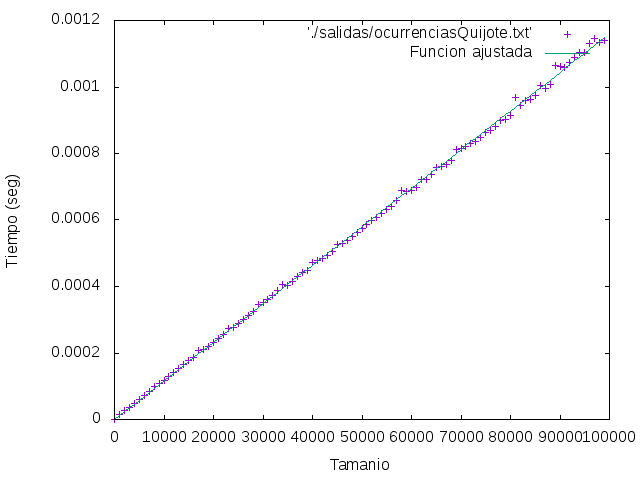
\includegraphics[width=12cm]{../salidas/ocurrenciasQuijote.png}
\end{center}
\end{figure}


\subsection{Considerando como entrada el texto del fichero lema.txt.}

Compilamos el código \texttt{ocurrencias.cpp} modificando el código para que lea y cuente las palabras del fichero \texttt{lema.txt}:
\begin{minted}{shell-session}
g++ -std=c++11 -o ./bin/ocurrencias ./src/ocurrencias.cpp
\end{minted}

Guardamos la salida de la ejecución en un fichero llamado \texttt{ocurrenciasDicc.txt}, donde la primera columna representa el tamaño del conjunto de palabras y la segunda el tiempo necesario para buscar la palabra ``hidalgo":
\begin{minted}{shell-session}
./bin/ocurrencias > ./salidas/ocurrenciasDicc.txt
\end{minted}

Realizamos el enfoque híbrido con el ajuste de los datos obtenidos. Para hacer la regresión con \texttt{gnuplot} he definido la función $f(x) = a * x$, ya que el algoritmo tiene orden de eficiencia $O(n)$.

\begin{minted}{shell-session}
gnuplot> plot './salidas/ocurrenciasDicc.txt' title 'Eficiencia ocurrencia Diccionario' 
with points
gnuplot> set xlabel "Tamanio"
gnuplot> set ylabel "Tiempo (seg)"
gnuplot> f(x) = a * x
gnuplot> fit f(x) './salidas/ocurrenciasDicc.txt' via a

Final set of parameters            Asymptotic Standard Error
=======================            ==========================
a               = 1.28826e-08      +/- 2.827e-11    (0.2194%)

gnuplot> plot './salidas/ocurrenciasDicc.txt', f(x) title 'Funcion ajustada'
\end{minted}

\begin{figure}[H]
\begin{center}
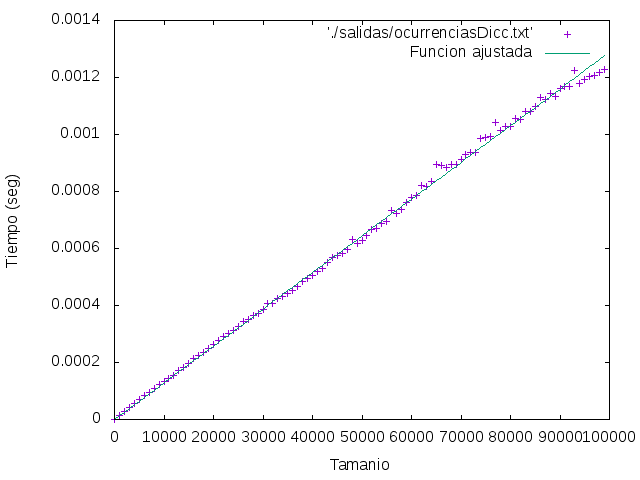
\includegraphics[width=12cm]{../salidas/ocurrenciasDicc.png}
\end{center}
\end{figure}


\section{Análisis de eficiencia del código en frecuencias.cpp, considerando como entradas el texto del fichero quijote.txt.}

Para realizar el cálculo empírico de la eficiencia del algoritmo, hemos ejecutado el programa en un ordenador cuyas prestaciones son: procesador Intel Core i7 con 6GB de RAM, y el compilador empleado es `g++'.\\

Para poder realizar bien el ejercicio modificamos el código para poder guardar en un fichero distinto las salidas de las distintas versiones de \texttt{contar\_frecuencias}. Para compilar el código utilizamos:
\begin{minted}{shell-session}
g++ -std=c++11 -o ./bin/frecuencias ./src/frecuencias.cpp 
\end{minted}

Guardamos las distintas salidas de las ejecuciones en ficheros llamados \texttt{frecuenciasV1.txt},\\ \texttt{frecuenciasV2.txt}, \texttt{frecuenciasV3.txt}, \texttt{frecuenciasV4.txt}, donde la primera columna representa el tamaño del conjunto de palabras y la segunda el tiempo transcurrido:
\begin{minted}{shell-session}
./bin/ocurrencias > ./salidas/frecuencias.txt
\end{minted}

\subsection{Análisis de eficiencia del código con la estructura de datos de la versión 1.}

\begin{minted}{c++}
int contar_hasta( vector<string> & V, int ini, int fin, string & s) {
   int cuantos = 0;
   for (int i=ini; i< fin ; i++)
      if (V[i]==s) {
         cuantos ++;
      }
   return cuantos;
}


void contar_frecuencias_V1( vector<string> & libro, int ini, int fin,
                         vector<string> &pal, vector<int> & frec ){
   int cuantas;
   for (int i = ini; i<fin; i++){

      cuantas = contar_hasta(libro,ini,fin,libro[i]); //O(n)
      pal.push_back(libro[i]); //tiempo amortizado O(1)
      frec.push_back(cuantas); //tiempo amortizado O(1)
   }
}
\end{minted}

El método \texttt{contar\_hasta} es del orden $O(n)$ y el método \texttt{push\_back }del vector es $0(1)$, por lo tanto \texttt{contar\_frecuencias\_V1} es del orden $O(n^2)$.\\

Realizamos el enfoque híbrido con el ajuste de los datos obtenidos. Para hacer la regresión con \texttt{gnuplot} he definido la función $f(x) = a * x * x$, ya que el algoritmo tiene orden de eficiencia $O(n^2)$.

\begin{minted}{shell-session}
gnuplot> plot './salidas/frecuenciasV1.txt' title 'Eficiencia frecuenciasV1' 
with points
gnuplot> set xlabel "Tamanio"
gnuplot> set ylabel "Tiempo (seg)"
gnuplot> f(x) = a * x * x
gnuplot> fit f(x) './salidas/frecuenciasV1.txt' via a

Final set of parameters            Asymptotic Standard Error
=======================            ==========================
a               = 1.2061e-08       +/- 2.999e-11    (0.2487%)

gnuplot> plot './salidas/frecuenciasV1.txt', f(x) title 'Funcion ajustada'
\end{minted}

\begin{figure}[H]
\begin{center}
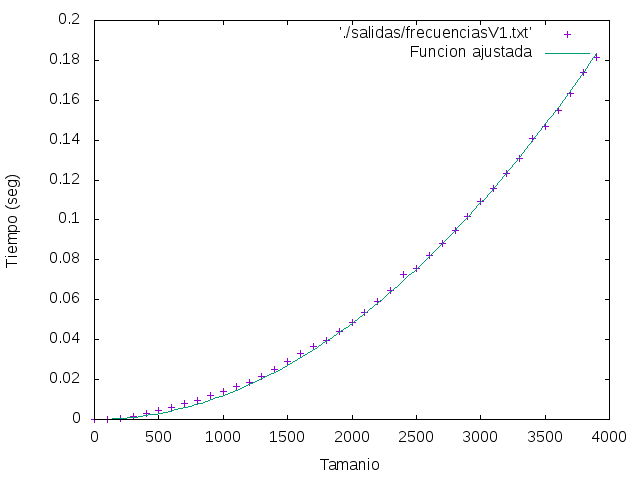
\includegraphics[width=12cm]{../salidas/frecuenciasV1.png}
\end{center}
\end{figure}

\subsection{Análisis de eficiencia del código con la estructura de datos de la versión 2.}

\begin{minted}{c++}
int buscar( vector<string> & V, string & s) {
   bool enc= false;
   int pos = POS_NULA;
   for (int i=0; i< V.size() && !enc; i++)
      if (V[i]==s) {
         enc = true;
         pos = i;
      }
   return pos;
}


void contar_frecuencias_V2( vector<string> & libro, int ini, int fin,
                         vector<string> &pal, vector<int> & frec ){
   int pos;
   for (int i = ini; i<fin; i++){

      pos = buscar(pal, libro[i]); // O(n)
      if (pos==POS_NULA) {
         pal.push_back(libro[i]);    // Análisis amortizado O(1)
         frec.push_back(1);    // Análisis amortizado O(1)
      }
      else {
         frec[pos]++;
      }

   }
}
\end{minted}

El método \texttt{buscar} es del orden $O(n)$ y el método \texttt{push\_back }del vector es $0(1)$, por lo tanto \texttt{contar\_frecuencias\_V2} es del orden $O(n^2)$.\\

Realizamos el enfoque híbrido con el ajuste de los datos obtenidos. Para hacer la regresión con \texttt{gnuplot} he definido la función $f(x) = a * x * x$, ya que el algoritmo tiene orden de eficiencia $O(n^2)$.

\begin{minted}{shell-session}
gnuplot> plot './salidas/frecuenciasV2.txt' title 'Eficiencia frecuenciasV2' 
with points
gnuplot> set xlabel "Tamanio"
gnuplot> set ylabel "Tiempo (seg)"
gnuplot> f(x) = a * x * x
gnuplot> fit f(x) './salidas/frecuenciasV2.txt' via a

Final set of parameters            Asymptotic Standard Error
=======================            ==========================
a               = 1.37174e-09      +/- 1.585e-11    (1.156%)

gnuplot> plot './salidas/frecuenciasV2.txt', f(x) title 'Funcion ajustada'
\end{minted}

\begin{figure}[H]
\begin{center}
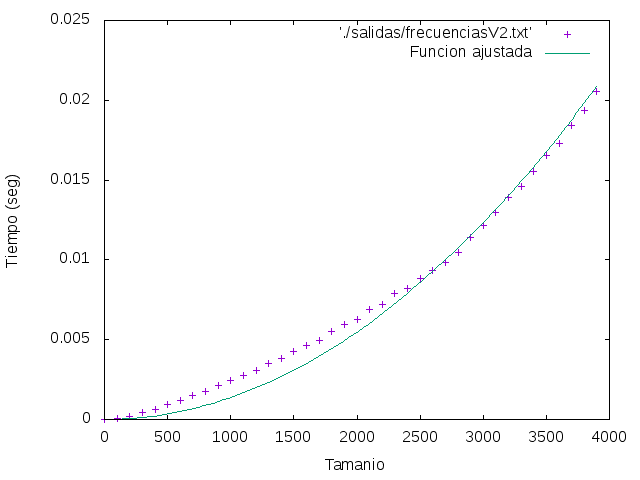
\includegraphics[width=12cm]{../salidas/frecuenciasV2.png}
\end{center}
\end{figure}


\subsection{Análisis de eficiencia del código con la estructura de datos de la versión 3.}

\begin{minted}{c++}
void contar_frecuencias_V3( vector<string> & libro, int ini, int fin,
                         vector<string> &pal, vector<int> & frec ){
   vector<string>::iterator pos;
   for (int i = ini; i<fin; i++){

      pos = lower_bound(pal.begin(), pal.end(), libro[i]);  // O(log (n) )
      					// n tama del vector  Busqueda Binaria
      if ((pos==pal.end()) || (*pos!=libro[i])) {
         frec.insert(frec.begin() + (pos-pal.begin()), 1);   //O(n)
         pal.insert(pos, libro[i]);            //O (n)
      }
      else {
         frec[pos-pal.begin()]++; // O(1)
      }

   }
}
\end{minted}


La eficiencia en el interior del bucle for es $O(log (n) + n) = O(n)$, por lo tanto el método\\ \texttt{contar\_frecuencias\_V3} es del orden $O(n^2)$.\\

Realizamos el enfoque híbrido con el ajuste de los datos obtenidos. Para hacer la regresión con \texttt{gnuplot} he definido la función $f(x) = a * x * x$, ya que el algoritmo tiene orden de eficiencia $O(n^2)$.

\begin{minted}{shell-session}
gnuplot> plot './salidas/frecuenciasV3.txt' title 'Eficiencia frecuenciasV3' 
with points
gnuplot> set xlabel "Tamanio"
gnuplot> set ylabel "Tiempo (seg)"
gnuplot> f(x) = a * x * x
gnuplot> fit f(x) './salidas/frecuenciasV3.txt' via a

Final set of parameters            Asymptotic Standard Error
=======================            ==========================
a               = 4.14655e-10      +/- 1.11e-11     (2.676%)

gnuplot> plot './salidas/frecuenciasV3.txt', f(x) title 'Funcion ajustada'
\end{minted}

\begin{figure}[H]
\begin{center}
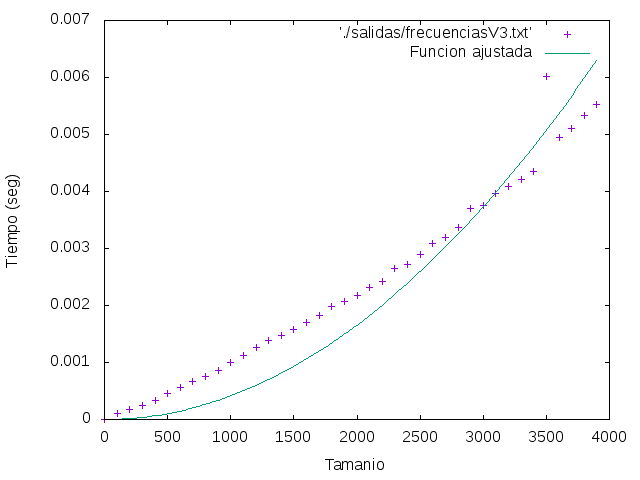
\includegraphics[width=12cm]{../salidas/frecuenciasV3.png}
\end{center}
\end{figure}

\subsection{Análisis de eficiencia del código con la estructura de datos de la versión 4.}

\begin{minted}{c++}
void contar_frecuencias_V4( vector<string> & libro, int ini, int fin,
                         vector<string> &pal, vector<int> & frec ){

   map<string,int> M;
   for (int i = ini; i<fin; i++)
      M[libro[i]]++;         // O( log(n) )

   map<string,int>::iterator it;
   for (it = M.begin(); it!= M.end(); ++ it){ // Bucle O(k log k) siendo k el 
   					   //numero de palabras distintas
      pal.push_back( (*it).first ); //O(1)
      frec.push_back( (*it).second ); //O(1)
   }
}
\end{minted}


La eficiencia del primer bucle for es $O(n log (n))$,la eficiencia del segundo bucle for es $O(n log(n))$, por lo tanto el método \texttt{contar\_frecuencias\_V4} es del orden $O(n log(n))$.\\

Realizamos el enfoque híbrido con el ajuste de los datos obtenidos. Para hacer la regresión con \texttt{gnuplot} he definido la función $f(x) = a * x$, aunque teóricamente el algoritmo tiene orden de eficiencia $O(n log(n))$, se puede observar que el ajuste a $f(x) = a * x$ es mucho más exacto.

\begin{minted}{shell-session}
gnuplot> plot './salidas/frecuenciasV4.txt' title 'Eficiencia frecuenciasV4' 
with points
gnuplot> set xlabel "Tamanio"
gnuplot> set ylabel "Tiempo (seg)"
gnuplot> f(x) = a * x
gnuplot> fit f(x) './salidas/frecuenciasV4.txt' via a

Final set of parameters            Asymptotic Standard Error
=======================            ==========================
a               = 6.71595e-07      +/- 1.725e-09    (0.2569%)

gnuplot> plot './salidas/frecuenciasV4.txt', f(x) title 'Funcion ajustada'
\end{minted}

\begin{figure}[H]
\begin{center}
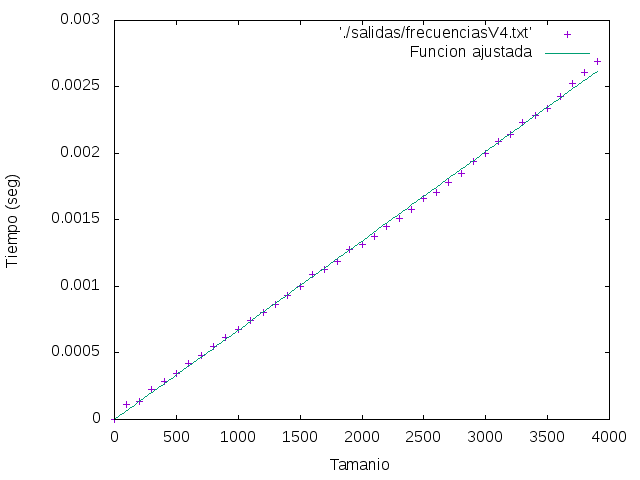
\includegraphics[width=12cm]{../salidas/frecuenciasV4.png}
\end{center}
\end{figure}

\section{Realizar el análisis de eficiencia teórico y práctico con los algoritmos de ordenación que se conocen (burbuja, inserción y selección).}

Para realizar el cálculo empírico de la eficiencia del algoritmo, hemos ejecutado el programa en un ordenador cuyas prestaciones son: procesador Intel Core i7 con 6GB de RAM, y el compilador empleado es `g++'.\\

\subsection{Burbuja}
Para compilar el código utilizamos:
\begin{minted}{shell-session}
g++ -std=c++11 -o ./bin/BurbujaEficiencia ./src/BurbujaEficiencia_Lims.cpp 
\end{minted}

Guardamos la salida del programa en un fichero llamado \texttt{ordenacionBurbuja.txt}, donde la primera columna representa el tamaño del conjunto de palabras y la segunda el tiempo transcurrido:
\begin{minted}{shell-session}
./bin/BurbujaEficiencia 0 10000 100 > ./salidas/ordenacionBurbuja.txt
\end{minted}

\begin{minted}{c++}
void burbuja(vector<int> & T, int inicial, int final)
{
 int i, j;
 int aux;
 for (i = inicial; i < final - 1; i++) //O(n^2)
   for (j = final - 1; j > i; j--) //O(n)
       if (T[j] < T[j-1])
         {
           aux = T[j];  //O(1)
           T[j] = T[j-1]; //O(1)
           T[j-1] = aux; //O(1)
         }
}
\end{minted}

La eficiencia de ordenación mediante burbuja es $O(n^2)$.

Realizamos el enfoque híbrido con el ajuste de los datos obtenidos. Para hacer la regresión con \texttt{gnuplot} he definido la función $f(x) = a * x * x$.

\begin{minted}{shell-session}
gnuplot> plot './salidas/ordenacionBurbuja.txt' title 'Eficiencia ordenacionBurbuja' 
with points
gnuplot> set xlabel "Tamanio"
gnuplot> set ylabel "Tiempo (seg)"
gnuplot> f(x) = a * x * x
gnuplot> fit f(x) './salidas/ordenacionBurbuja.txt' via a

Final set of parameters            Asymptotic Standard Error
=======================            ==========================
a               = 7.05041e-09      +/- 3.095e-11    (0.439%)

gnuplot> plot './salidas/ordenacionBurbuja.txt', f(x) title 'Funcion ajustada'
\end{minted}

\begin{figure}[H]
\begin{center}
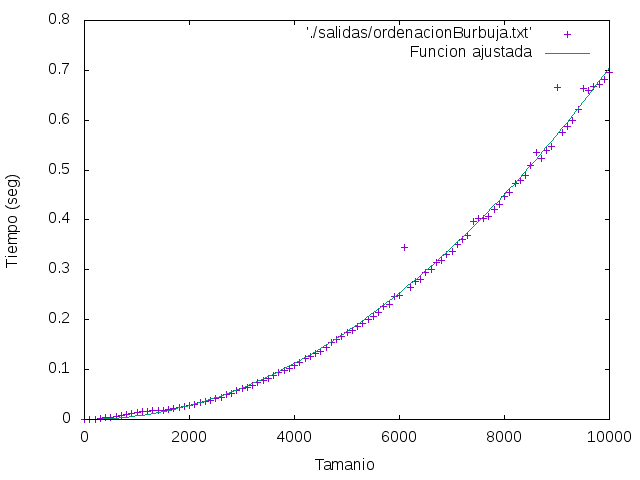
\includegraphics[width=12cm]{../salidas/ordenacionBurbuja.png}
\end{center}
\end{figure}

\subsection{Selección}

Para compilar el código utilizamos:
\begin{minted}{shell-session}
g++ -std=c++11 -o ./bin/SeleccionEficiencia ./src/SeleccionEficiencia.cpp 
\end{minted}

Guardamos la salida del programa en un fichero llamado \texttt{ordenacionSeleccion.txt}, donde la primera columna representa el tamaño del conjunto de palabras y la segunda el tiempo transcurrido:
\begin{minted}{shell-session}
./bin/SeleccionEficiencia > ./salidas/ordenacionSeleccion.txt
\end{minted}

\begin{minted}{c++}
void seleccion(vector<int> & T, int inicial, int final)
{
   int i, j,min,aux;
   for (i = inicial; i < final - 1; i++){ // O(n^2)
      min = i;
      for (j = i + 1; j < final ; j++) // O(n)
         if (T[j] < T[min]) // O(1)
            min=j; // O(1)
      aux = T[min]; // O(1)
      T[min] = T[i]; // O(1)
      T[i] = aux; // O(1)
   }
}
\end{minted}

La eficiencia de ordenación mediante selección es $O(n^2)$.

Realizamos el enfoque híbrido con el ajuste de los datos obtenidos. Para hacer la regresión con \texttt{gnuplot} he definido la función $f(x) = a * x * x$.

\begin{minted}{shell-session}
gnuplot> plot './salidas/ordenacionSeleccion.txt' title 'Eficiencia ordenacionSeleccion' 
with points
gnuplot> set xlabel "Tamanio"
gnuplot> set ylabel "Tiempo (seg)"
gnuplot> f(x) = a * x * x
gnuplot> fit f(x) './salidas/ordenacionSeleccion.txt' via a

Final set of parameters            Asymptotic Standard Error
=======================            ==========================
a               = 2.82297e-09      +/- 6.298e-12    (0.2231%)


gnuplot> plot './salidas/ordenacionSeleccion.txt', f(x) title 'Funcion ajustada'
\end{minted}

\begin{figure}[H]
\begin{center}
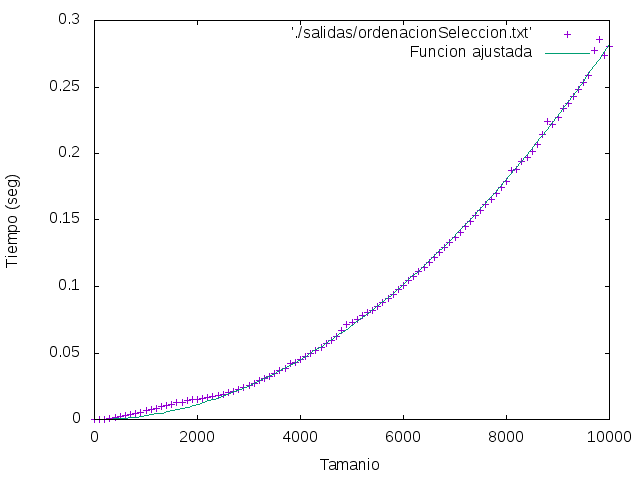
\includegraphics[width=12cm]{../salidas/ordenacionSeleccion.png}
\end{center}
\end{figure}


\subsection{Inserción}

Para compilar el código utilizamos:
\begin{minted}{shell-session}
g++ -std=c++11 -o ./bin/InsercionEficiencia ./src/InsercionEficiencia.cpp 
\end{minted}

Guardamos la salida del programa en un fichero llamado \texttt{ordenacionInsercion.txt}, donde la primera columna representa el tamaño del conjunto de palabras y la segunda el tiempo transcurrido:
\begin{minted}{shell-session}
./bin/InsercionEficiencia 0 10000 100> ./salidas/ordenacionInsercion.txt
\end{minted}

\begin{minted}{c++}
void insercion(vector<int> & T, int inicial, int final)
{
   int i, j,valor;
   for (i = inicial; i < final; i++){ O(n^2)
      valor = T[i];
      for (j = i ; j > 0 && T[j-1] > valor; j--) // O(n)
         T[j] = T[j-1];
      T[j] = valor;
   }
}
\end{minted}

La eficiencia de ordenación mediante inserción es $O(n^2)$.

Realizamos el enfoque híbrido con el ajuste de los datos obtenidos. Para hacer la regresión con \texttt{gnuplot} he definido la función $f(x) = a * x * x$.

\begin{minted}{shell-session}
gnuplot> plot './salidas/ordenacionInsercion.txt' title 'Eficiencia ordenacionInsercion' 
with points
gnuplot> set xlabel "Tamanio"
gnuplot> set ylabel "Tiempo (seg)"
gnuplot> f(x) = a * x * x
gnuplot> fit f(x) './salidas/ordenacionInsercion.txt' via a

Final set of parameters            Asymptotic Standard Error
=======================            ==========================
a               = 2.03009e-09      +/- 1.219e-11    (0.6006%)

gnuplot> plot './salidas/ordenacionInsercion.txt', f(x) title 'Funcion ajustada'
\end{minted}

\begin{figure}[H]
\begin{center}
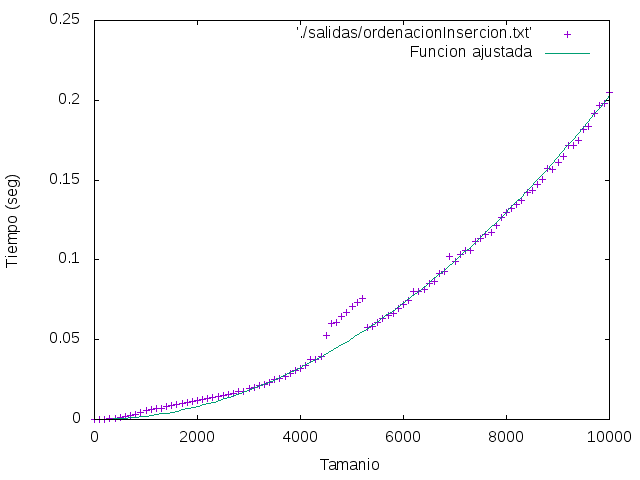
\includegraphics[width=12cm]{../salidas/ordenacionInsercion.png}
\end{center}
\end{figure}


\end{document}